% !TEX root = report.tex

%% bare_conf.tex
%% V1.3
%% 2007/01/11
%% by Michael Shell
%% See:
%% http://www.michaelshell.org/
%% for current contact information.
%%
%% This is a skeleton file demonstrating the use of IEEEtran.cls
%% (requires IEEEtran.cls version 1.7 or later) with an IEEE conference paper.
%%
%% Support sites:
%% http://www.michaelshell.org/tex/ieeetran/
%% http://www.ctan.org/tex-archive/macros/latex/contrib/IEEEtran/
%% and
%% http://www.ieee.org/

%%*************************************************************************
%% Legal Notice:
%% This code is offered as-is without any warranty either expressed or
%% implied; without even the implied warranty of MERCHANTABILITY or
%% FITNESS FOR A PARTICULAR PURPOSE!
%% User assumes all risk.
%% In no event shall IEEE or any contributor to this code be liable for
%% any damages or losses, including, but not limited to, incidental,
%% consequential, or any other damages, resulting from the use or misuse
%% of any information contained here.
%%
%% All comments are the opinions of their respective authors and are not
%% necessarily endorsed by the IEEE.
%%
%% This work is distributed under the LaTeX Project Public License (LPPL)
%% ( http://www.latex-project.org/ ) version 1.3, and may be freely used,
%% distributed and modified. A copy of the LPPL, version 1.3, is included
%% in the base LaTeX documentation of all distributions of LaTeX released
%% 2003/12/01 or later.
%% Retain all contribution notices and credits.
%% ** Modified files should be clearly indicated as such, including  **
%% ** renaming them and changing author support contact information. **
%%
%% File list of work: IEEEtran.cls, IEEEtran_HOWTO.pdf, bare_adv.tex,
%%                    bare_conf.tex, bare_jrnl.tex, bare_jrnl_compsoc.tex
%%*************************************************************************

% *** Authors should verify (and, if needed, correct) their LaTeX system  ***
% *** with the testflow diagnostic prior to trusting their LaTeX platform ***
% *** with production work. IEEE's font choices can trigger bugs that do  ***
% *** not appear when using other class files.                            ***
% The testflow support page is at:
% http://www.michaelshell.org/tex/testflow/



% Note that the a4paper option is mainly intended so that authors in
% countries using A4 can easily print to A4 and see how their papers will
% look in print - the typesetting of the document will not typically be
% affected with changes in paper size (but the bottom and side margins will).
% Use the testflow package mentioned above to verify correct handling of
% both paper sizes by the user's LaTeX system.
%
% Also note that the "draftcls" or "draftclsnofoot", not "draft", option
% should be used if it is desired that the figures are to be displayed in
% draft mode.
%
\documentclass[conference, letterpaper]{IEEEtran}
% Add the compsoc option for Computer Society conferences.
%
% If IEEEtran.cls has not been installed into the LaTeX system files,
% manually specify the path to it like:
% \documentclass[conference]{../sty/IEEEtran}





% Some very useful LaTeX packages include:
% (uncomment the ones you want to load)

\usepackage{listings}

% *** MISC UTILITY PACKAGES ***
%
%\usepackage{ifpdf}
% Heiko Oberdiek's ifpdf.sty is very useful if you need conditional
% compilation based on whether the output is pdf or dvi.
% usage:
% \ifpdf
%   % pdf code
% \else
%   % dvi code
% \fi
% The latest version of ifpdf.sty can be obtained from:
% http://www.ctan.org/tex-archive/macros/latex/contrib/oberdiek/
% Also, note that IEEEtran.cls V1.7 and later provides a builtin
% \ifCLASSINFOpdf conditional that works the same way.
% When switching from latex to pdflatex and vice-versa, the compiler may
% have to be run twice to clear warning/error messages.






% *** CITATION PACKAGES ***
%
%\usepackage{cite}
% cite.sty was written by Donald Arseneau
% V1.6 and later of IEEEtran pre-defines the format of the cite.sty package
% \cite{} output to follow that of IEEE. Loading the cite package will
% result in citation numbers being automatically sorted and properly
% "compressed/ranged". e.g., [1], [9], [2], [7], [5], [6] without using
% cite.sty will become [1], [2], [5]--[7], [9] using cite.sty. cite.sty's
% \cite will automatically add leading space, if needed. Use cite.sty's
% noadjust option (cite.sty V3.8 and later) if you want to turn this off.
% cite.sty is already installed on most LaTeX systems. Be sure and use
% version 4.0 (2003-05-27) and later if using hyperref.sty. cite.sty does
% not currently provide for hyperlinked citations.
% The latest version can be obtained at:
% http://www.ctan.org/tex-archive/macros/latex/contrib/cite/
% The documentation is contained in the cite.sty file itself.






% *** GRAPHICS RELATED PACKAGES ***
%
\ifCLASSINFOpdf
  % \usepackage[pdftex]{graphicx}
  % declare the path(s) where your graphic files are
  % \graphicspath{{../pdf/}{../jpeg/}}
  % and their extensions so you won't have to specify these with
  % every instance of \includegraphics
  % \DeclareGraphicsExtensions{.pdf,.jpeg,.png}
\else
  % or other class option (dvipsone, dvipdf, if not using dvips). graphicx
  % will default to the driver specified in the system graphics.cfg if no
  % driver is specified.
  % \usepackage[dvips]{graphicx}
  % declare the path(s) where your graphic files are
  % \graphicspath{{../eps/}}
  % and their extensions so you won't have to specify these with
  % every instance of \includegraphics
  % \DeclareGraphicsExtensions{.eps}
\fi
% graphicx was written by David Carlisle and Sebastian Rahtz. It is
% required if you want graphics, photos, etc. graphicx.sty is already
% installed on most LaTeX systems. The latest version and documentation can
% be obtained at:
% http://www.ctan.org/tex-archive/macros/latex/required/graphics/
% Another good source of documentation is "Using Imported Graphics in
% LaTeX2e" by Keith Reckdahl which can be found as epslatex.ps or
% epslatex.pdf at: http://www.ctan.org/tex-archive/info/
%
% latex, and pdflatex in dvi mode, support graphics in encapsulated
% postscript (.eps) format. pdflatex in pdf mode supports graphics
% in .pdf, .jpeg, .png and .mps (metapost) formats. Users should ensure
% that all non-photo figures use a vector format (.eps, .pdf, .mps) and
% not a bitmapped formats (.jpeg, .png). IEEE frowns on bitmapped formats
% which can result in "jaggedy"/blurry rendering of lines and letters as
% well as large increases in file sizes.
%
% You can find documentation about the pdfTeX application at:
% http://www.tug.org/applications/pdftex





% *** MATH PACKAGES ***
%
%\usepackage[cmex10]{amsmath}
% A popular package from the American Mathematical Society that provides
% many useful and powerful commands for dealing with mathematics. If using
% it, be sure to load this package with the cmex10 option to ensure that
% only type 1 fonts will utilized at all point sizes. Without this option,
% it is possible that some math symbols, particularly those within
% footnotes, will be rendered in bitmap form which will result in a
% document that can not be IEEE Xplore compliant!
%
% Also, note that the amsmath package sets \interdisplaylinepenalty to 10000
% thus preventing page breaks from occurring within multiline equations. Use:
%\interdisplaylinepenalty=2500
% after loading amsmath to restore such page breaks as IEEEtran.cls normally
% does. amsmath.sty is already installed on most LaTeX systems. The latest
% version and documentation can be obtained at:
% http://www.ctan.org/tex-archive/macros/latex/required/amslatex/math/





% *** SPECIALIZED LIST PACKAGES ***
%
%\usepackage{algorithmic}
% algorithmic.sty was written by Peter Williams and Rogerio Brito.
% This package provides an algorithmic environment fo describing algorithms.
% You can use the algorithmic environment in-text or within a figure
% environment to provide for a floating algorithm. Do NOT use the algorithm
% floating environment provided by algorithm.sty (by the same authors) or
% algorithm2e.sty (by Christophe Fiorio) as IEEE does not use dedicated
% algorithm float types and packages that provide these will not provide
% correct IEEE style captions. The latest version and documentation of
% algorithmic.sty can be obtained at:
% http://www.ctan.org/tex-archive/macros/latex/contrib/algorithms/
% There is also a support site at:
% http://algorithms.berlios.de/index.html
% Also of interest may be the (relatively newer and more customizable)
% algorithmicx.sty package by Szasz Janos:
% http://www.ctan.org/tex-archive/macros/latex/contrib/algorithmicx/




% *** ALIGNMENT PACKAGES ***
%
%\usepackage{array}
% Frank Mittelbach's and David Carlisle's array.sty patches and improves
% the standard LaTeX2e array and tabular environments to provide better
% appearance and additional user controls. As the default LaTeX2e table
% generation code is lacking to the point of almost being broken with
% respect to the quality of the end results, all users are strongly
% advised to use an enhanced (at the very least that provided by array.sty)
% set of table tools. array.sty is already installed on most systems. The
% latest version and documentation can be obtained at:
% http://www.ctan.org/tex-archive/macros/latex/required/tools/


%\usepackage{mdwmath}
%\usepackage{mdwtab}
% Also highly recommended is Mark Wooding's extremely powerful MDW tools,
% especially mdwmath.sty and mdwtab.sty which are used to format equations
% and tables, respectively. The MDWtools set is already installed on most
% LaTeX systems. The lastest version and documentation is available at:
% http://www.ctan.org/tex-archive/macros/latex/contrib/mdwtools/


% IEEEtran contains the IEEEeqnarray family of commands that can be used to
% generate multiline equations as well as matrices, tables, etc., of high
% quality.


%\usepackage{eqparbox}
% Also of notable interest is Scott Pakin's eqparbox package for creating
% (automatically sized) equal width boxes - aka "natural width parboxes".
% Available at:
% http://www.ctan.org/tex-archive/macros/latex/contrib/eqparbox/

% *** SUBFIGURE PACKAGES ***
%\usepackage[tight,footnotesize]{subfigure}
% subfigure.sty was written by Steven Douglas Cochran. This package makes it
% easy to put subfigures in your figures. e.g., "Figure 1a and 1b". For IEEE
% work, it is a good idea to load it with the tight package option to reduce
% the amount of white space around the subfigures. subfigure.sty is already
% installed on most LaTeX systems. The latest version and documentation can
% be obtained at:
% http://www.ctan.org/tex-archive/obsolete/macros/latex/contrib/subfigure/
% subfigure.sty has been superceeded by subfig.sty.

%\usepackage[caption=false]{caption}
%\usepackage[font=footnotesize]{subfig}
% subfig.sty, also written by Steven Douglas Cochran, is the modern
% replacement for subfigure.sty. However, subfig.sty requires and
% automatically loads Axel Sommerfeldt's caption.sty which will override
% IEEEtran.cls handling of captions and this will result in nonIEEE style
% figure/table captions. To prevent this problem, be sure and preload
% caption.sty with its "caption=false" package option. This is will preserve
% IEEEtran.cls handing of captions. Version 1.3 (2005/06/28) and later
% (recommended due to many improvements over 1.2) of subfig.sty supports
% the caption=false option directly:
%\usepackage[caption=false,font=footnotesize]{subfig}
%
% The latest version and documentation can be obtained at:
% http://www.ctan.org/tex-archive/macros/latex/contrib/subfig/
% The latest version and documentation of caption.sty can be obtained at:
% http://www.ctan.org/tex-archive/macros/latex/contrib/caption/

% *** FLOAT PACKAGES ***
%
%\usepackage{fixltx2e}
% fixltx2e, the successor to the earlier fix2col.sty, was written by
% Frank Mittelbach and David Carlisle. This package corrects a few problems
% in the LaTeX2e kernel, the most notable of which is that in current
% LaTeX2e releases, the ordering of single and double column floats is not
% guaranteed to be preserved. Thus, an unpatched LaTeX2e can allow a
% single column figure to be placed prior to an earlier double column
% figure. The latest version and documentation can be found at:
% http://www.ctan.org/tex-archive/macros/latex/base/

%\usepackage{stfloats}
% stfloats.sty was written by Sigitas Tolusis. This package gives LaTeX2e
% the ability to do double column floats at the bottom of the page as well
% as the top. (e.g., "\begin{figure*}[!b]" is not normally possible in
% LaTeX2e). It also provides a command:
%\fnbelowfloat
% to enable the placement of footnotes below bottom floats (the standard
% LaTeX2e kernel puts them above bottom floats). This is an invasive package
% which rewrites many portions of the LaTeX2e float routines. It may not work
% with other packages that modify the LaTeX2e float routines. The latest
% version and documentation can be obtained at:
% http://www.ctan.org/tex-archive/macros/latex/contrib/sttools/
% Documentation is contained in the stfloats.sty comments as well as in the
% presfull.pdf file. Do not use the stfloats baselinefloat ability as IEEE
% does not allow \baselineskip to stretch. Authors submitting work to the
% IEEE should note that IEEE rarely uses double column equations and
% that authors should try to avoid such use. Do not be tempted to use the
% cuted.sty or midfloat.sty packages (also by Sigitas Tolusis) as IEEE does
% not format its papers in such ways.

% *** PDF, URL AND HYPERLINK PACKAGES ***
%
%\usepackage{url}
% url.sty was written by Donald Arseneau. It provides better support for
% handling and breaking URLs. url.sty is already installed on most LaTeX
% systems. The latest version can be obtained at:
% http://www.ctan.org/tex-archive/macros/latex/contrib/misc/
% Read the url.sty source comments for usage information. Basically,
% \url{my_url_here}.

% *** Do not adjust lengths that control margins, column widths, etc. ***
% *** Do not use packages that alter fonts (such as pslatex).         ***
% There should be no need to do such things with IEEEtran.cls V1.6 and later.
% (Unless specifically asked to do so by the journal or conference you plan
% to submit to, of course. )


% correct bad hyphenation here
\hyphenation{op-tical net-works semi-conduc-tor}

%\usepackage{subcaption}

% *** GRAPHICS RELATED PACKAGES ***
%
\ifCLASSINFOpdf
   \usepackage[pdftex]{graphicx}
\else
\fi

% *** MATH PACKAGES ***
%
\usepackage[cmex10]{amsmath}
\usepackage{color}
\usepackage[dvipsnames]{xcolor}
\usepackage{fancyhdr}
\usepackage[caption=false,font=footnotesize]{subfig}

\renewcommand{\thispagestyle}[2]{}

\fancypagestyle{plain}{
        \fancyhead{}
        \fancyhead[C]{first page center header}
        \fancyfoot{}
        \fancyfoot[C]{first page center footer}
}
\pagestyle{fancy}


\headheight 31.99992pt
\footskip 20pt

\rhead{}

%Enter the first page number of your paper below
\setcounter{page}{1}

%Header
% \fancyhead[R]{\textit{Capstone Report ~\textbullet~ 2171}}
% \fancyfoot[C]{\textit{RIT Computer Science}}
\fancyhead[R]{\textit{RIT Computer Science ~\textbullet~ Capstone Report ~\textbullet~ 20195}}
\renewcommand{\headrulewidth}{0pt}

%Footer
\fancyfoot[C]{Rochester Institute of Technology}
\renewcommand{\footrulewidth}{0.5pt}
\fancyfoot[R]{\thepage \  $|$ P a g e }


\begin{document}

%
% paper title
% can use linebreaks \\ within to get better formatting as desired
\title{Loom: One Web Development Tool for Everyone}


% author names and affiliations
% use a multiple column layout for up to three different
% affiliations
\ifx \isAnonymous \undefined
\author{\IEEEauthorblockN{Kyle Cutler}
\IEEEauthorblockA{Department of Computer Science\\Golisano College of Computing and Information Sciences\\
Rochester Institute of Technology\\
Rochester, NY 14623\\
kjc9861@cs.rit.edu}}
\fi


% make the title area
\maketitle


\begin{abstract}
Loom is a desktop application designed to bridge the gap between beginner and expert web development tools. Existing tools in the domain provide either easy-to-use interfaces intended for novice users, sacrificing expressiveness, or advanced interfaces which are intended for developers who already know web technologies, but are inaccessible by ordinary users. Loom is a first-of-its-kind tool that provides novice users the full power of web technologies such as HTML and CSS without the need to write code. In addition, Loom aims to impart the basics of these technologies to users as they work with the tool, teaching valuable concepts that can be carried over to other tools.
\end{abstract}

% \begin{IEEEkeywords}
% Keyword1; Keyword2; Keyword3
% \end{IEEEkeywords}


\IEEEpeerreviewmaketitle



\section{Introduction}
There are many existing web-development tools intended for a wide range of users. Some of these tools are targeted at novice users, and provide very easy-to-use interfaces with high-level features such as drag-and-drop and WYSIWYG editing. Other tools are intended for developers, and provide textual interfaces for working with code. Others still are intended for designers and may not support web technologies at all. The separation of these tools and the incompatibilities between them lead to several problems:
\begin{itemize}
    \item Coordination between these groups is difficult. If a novice user using a tool such as Wix\cite{Wix} or Squarespace\cite{Squarespace} decides they need a developer to continue their work, existing work will likely be wasted as the developer chooses to use a different tool.
    \item The work done by designers in tools such as Figma\cite{Figma}, Sketch\cite{Sketch} or InVision\cite{InVision} has to be mirrored by developers, wasting effort.
    \item Novice users are learning how to use a specific tool -- not the underlying technologies. Experience with one tool often does not carry over to others.
\end{itemize}

Some tools try to target more than one type of user. For example, WordPress\cite{WordPress} has a code editor, enabling developers to directly edit HTML code. Blocs\cite{Blocs}, a desktop application, provides designer-friendly tools, WYSIWYG editing and templates for beginners, and code editing for developers. But one problem with these tools still remains: novice users may never learn how to use "advanced" features such as code editing without doing their own research into web development.


\section{Approach}
Loom takes a different approach from most existing tools. It provides one common interface which is closely related to the underlying web technologies. This way, every user has the potential to use the full power of these technologies. The remaining challenge is making the interface intuitive to beginners, and familiar to developers and designers. To accomplish this, Loom uses a few strategies:
\begin{itemize}
  \item \textbf{Provide helpful, simple abstractions over existing technologies:} working directly with web technologies can be frustrating, even for developers. Loom aims to provide a handful of simple, but useful, abstractions over these technologies to make working with them easier.
  \item \textbf{Provide a user interface that "scales" with the user:} The interface should be easy for novices to pick up, but provide the full power for those who want it. For example, WYSIWYG editing and graphical components such as color pickers should make styling easy for beginners, but developers should be able to enter textual values for these properties as well.
\end{itemize}

% TODO: add section of different kinds of users here
% \subsection{User Categories}
% To accomplish the goal of providing a tool that can work for "everyone", we first define the different categories of users targeted by Loom. These categories may overlap, but each have a different set of needs.

Loom has the following motivating goals:

\subsection{Powerful}
Loom strives to give users the full power of the underlying technologies. For example, the user has the ability to use arbitrary HTML tags and attributes, use the full range of CSS selectors, or other advanced features. These features may not all necessarily have beginner-friendly interfaces, but should be accessible and intuitive to developers.

\subsection{Unified}
Loom's tagline is "one web development tool for everyone". But everyone has different needs. For example, designers are most interested in fast prototyping and easy styling tools, but developers will be concerned with the underlying workings of the site and modifying those in detail, and novice users will be focused on just learning the basics. In addition, a user may find themselves taking on multiple different roles -- for example, a developer who is also learning web technologies -- in which case, they should have total control over the page, but also guidance as to how to change every aspect of the content. So Loom must accommodate each user's needs, while remaining intuitive to those with different needs. This is the motivation behind Loom's "scaling" user interface.

\subsection{Educational}
For users who are not familiar with web technologies, Loom aims to be a tool they can use to learn these technologies. This includes both technical and non-technical users. For example, Loom should provide help with HTML and CSS whenever possible, and provide context clues and familiar interfaces to help the user make associations between the actions they perform and the resulting content changes.

\subsection{Simple}
Loom should be easy for anyone to learn to use. This includes novice users all the way to experienced developers. We do however assume a basic working knowledge of how to use a computer -- for example, users with basic proficiency in using a web browser.

% An example of a floating figure using the graphicx package.
% Note that \label must occur AFTER (or within) \caption.
% For figures, \caption should occur after the \includegraphics.
% Note that IEEEtran v1.7 and later has special internal code that
% is designed to preserve the operation of \label within \caption
% even when the captionsoff option is in effect. However, because
% of issues like this, it may be the safest practice to put all your
% \label just after \caption rather than within \caption{}.
%
% Reminder: the "draftcls" or "draftclsnofoot", not "draft", class
% option should be used if it is desired that the figures are to be
% displayed while in draft mode.
%

% A image is shown in Figure~\ref{fig:myfigure}.
% A citation\cite{IEEEexample:article_typical}.

% \begin{figure}[!t]
% \centering
% \includegraphics[width=2.5in]{myfigure}
% % where an .eps filename suffix will be assumed under latex,
% % and a .pdf suffix will be assumed for pdflatex; or what has been declared
% % via \DeclareGraphicsExtensions.
% \caption{Simulation Results}
% \label{fig:myfigure}
% \end{figure}


% In Listing~\ref{hw} a HelloWorld program is shown.

% \begin{lstlisting}[caption=writer.c., label=hw]
% int main() {
%   char * msg = "Hello World\n";
%   write(STDIN_FILENO, msg, strlen(msg));
%   exit(0);
% }
% \end{lstlisting}

% Note that IEEE typically puts floats only at the top, even when this
% results in a large percentage of a column being occupied by floats.


% An example of a double column floating figure using two subfigures.
% (The subfig.sty package must be loaded for this to work.)
% The subfigure \label commands are set within each subfloat command, the
% \label for the overall figure must come after \caption.
% \hfil must be used as a separator to get equal spacing.
% The subfigure.sty package works much the same way, except \subfigure is
% used instead of \subfloat.
%
%\begin{figure*}[!t]
%\centerline{\subfloat[Case I]\includegraphics[width=2.5in]{subfigcase1}%
%\label{fig_first_case}}
%\hfil
%\subfloat[Case II]{\includegraphics[width=2.5in]{subfigcase2}%
%\label{fig_second_case}}}
%\caption{Simulation results}
%\label{fig_sim}
%\end{figure*}
%
% Note that often IEEE papers with subfigures do not employ subfigure
% captions (using the optional argument to \subfloat), but instead will
% reference/describe all of them (a), (b), etc., within the main caption.


% An example of a floating table. Note that, for IEEE style tables, the
% \caption command should come BEFORE the table. Table text will default to
% \footnotesize as IEEE normally uses this smaller font for tables.
% The \label must come after \caption as always.
%
%\begin{table}[!t]
%% increase table row spacing, adjust to taste
%\renewcommand{\arraystretch}{1.3}
% if using array.sty, it might be a good idea to tweak the value of
% \extrarowheight as needed to properly center the text within the cells
%\caption{An Example of a Table}
%\label{table_example}
%\centering
%% Some packages, such as MDW tools, offer better commands for making tables
%% than the plain LaTeX2e tabular which is used here.
%\begin{tabular}{|c||c|}
%\hline
%One & Two\\
%\hline
%Three & Four\\
%\hline
%\end{tabular}
%\end{table}


% Note that IEEE does not put floats in the very first column - or typically
% anywhere on the first page for that matter. Also, in-text middle ("here")
% positioning is not used. Most IEEE journals/conferences use top floats
% exclusively. Note that, LaTeX2e, unlike IEEE journals/conferences, places
% footnotes above bottom floats. This can be corrected via the \fnbelowfloat
% command of the stfloats package.

\section{Design}
To accomplish its goals, Loom must have a logical design that allows users to create and edit every aspect of a website. There are three top-level types of objects the user can modify with Loom: Pages, Components, and Styles. Figure \ref{fig:design} shows the relationships between the different kinds of objects.

\begin{figure}[!t]
  \centering
  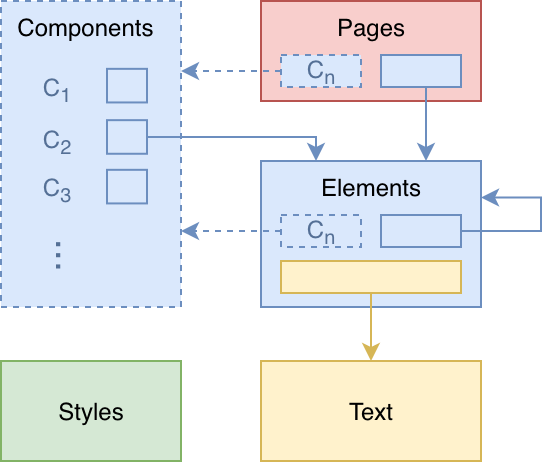
\includegraphics[width=2in]{../design.png}
  \caption{Relationships between each kind of object within Loom.}
  \label{fig:design}
\end{figure}

\subsection{Pages}
Loom aims to give users the ability to create entire static websites. The ability to create multiple pages is essential to this goal and is therefore one of the fundamental features in Loom. The user has the ability to create and name many different pages within a project. Each page represents a separate HTML page within the site.

Following standard HTML practices, in Loom all pages contain two elements nested within a root \texttt{html} element: a \texttt{head} and a \texttt{body}. Loom gives users the ability to modify these elements and their children by setting attributes, and creating and deleting elements and text content.

Elements are standard HTML elements -- consisting of a tag, zero or more attributes, and zero or more child elements or text. Therefore page contents form a tree-like structure just like standard HTML.

\subsection{Components}
In standard HTML, every Element belongs to just one parent. Thus there is no concept of "reusable" Elements in pure HTML – if you want multiple identical elements, you have to repeat yourself. This quickly becomes a pain to manage, especially across many pages. Loom includes the ability to create reusable elements by the name of "Components". Components are essentially just named Elements which can be reused across pages.

One common use case for components is to implement a site header and footer. Most websites reuse a header and footer across all pages. These often include things like navigation, a site logo, and contact information. In plain HTML, there is no way to reuse these across several pages without duplicating their entire HTML contents. But with Loom, the user can create components for the "header" and "footer", and then include them in several pages. Any changes to these components will then immediately be reflected across all pages using them. In a way, there are two "halves" to components: the definition, which associates an element with a given name, and references, which look up the component of a given name and insert its element in their place.

In Loom, the user has the ability to create new Components, update their contents and properties (just like any Element), and reference them from another Page or Component.

\subsection{Styles}
In general, every HTML Page can "link" to one or more CSS Stylesheets, whose styles will then be applied to that Page. However, this requires management of every page, ensuring that the correct Stylesheets are included for any elements on that page. In combination with components, it can become difficult to track which Stylesheets must be included on each page.

Loom simplifies this by using one shared Stylesheet across the entire project / website. This Stylesheet will be used by every page, and contains the styles for every Component. This greatly simplifies the management needed to ensure the correct styles get used on each page, but it also means the Stylesheet can become large and complex. The UI compensates for this by providing mechanisms to help the user easily find the style rules they are looking for, such as only showing styles applicable to a selected element. Note that this simplification can also be considered a drawback: splitting styles across multiple stylesheets can improve code organization and modularity, and would likely be a desirable feature for developers. Adding the ability to edit multiple stylesheets is an item for future work.

Loom gives the user the ability to create, delete, and update style rules in order to style the elements in the website. These rules use standard CSS syntax, and Loom provides simplified interfaces for working with many of the properties CSS provides.

\section{UI Design}
For Loom to accomplish its goals, it must have a sensibly designed UI. The UI of Loom is divided into three main sections: the Navigator, the WYSIWYG Editor, and the Properties Editor.

\begin{figure}[!t]
  \centering
  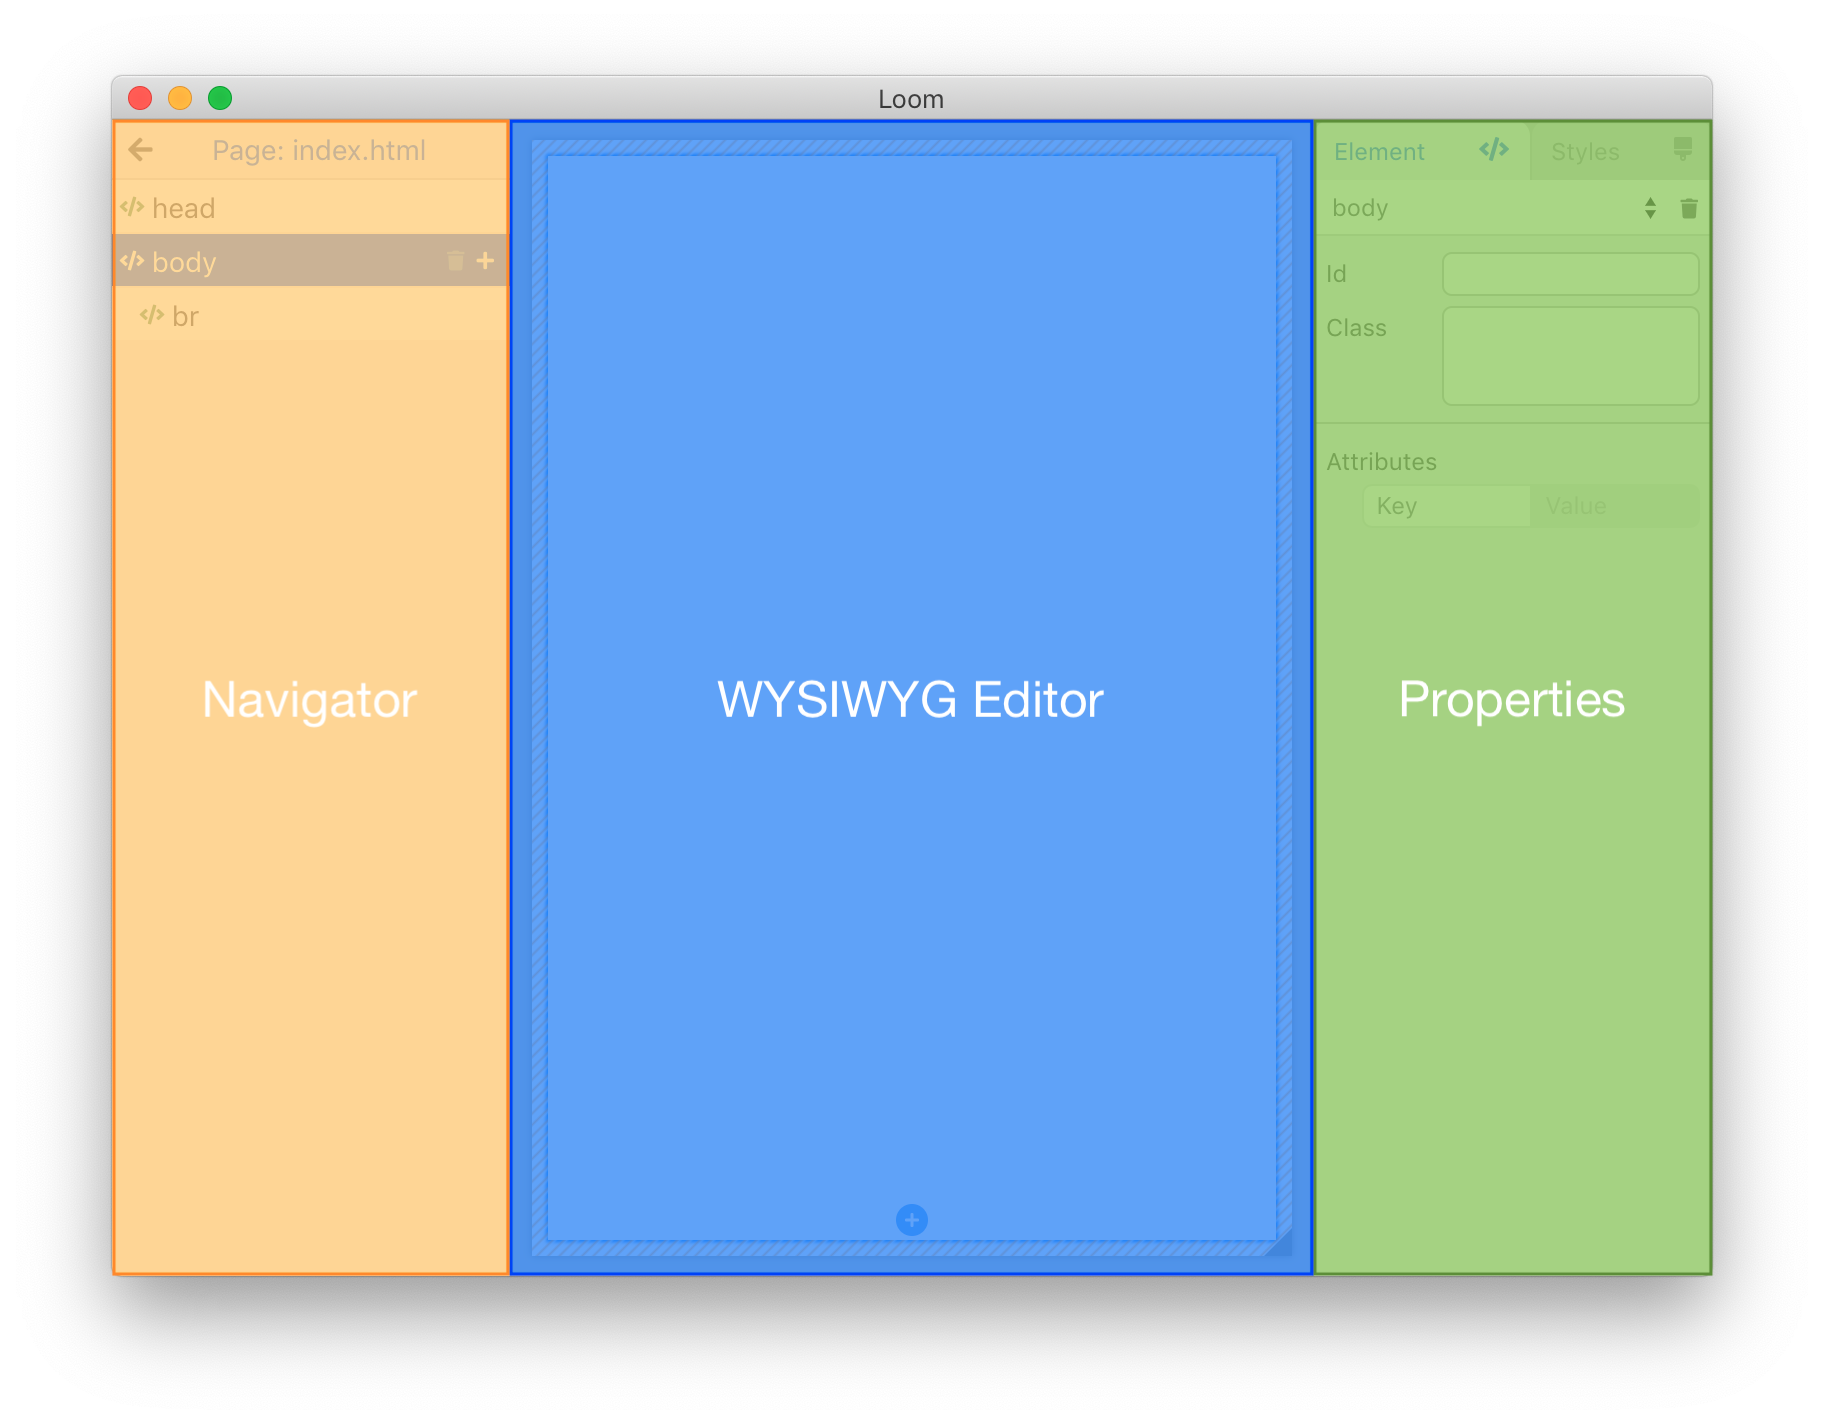
\includegraphics[width=3in]{../ui_outline.png}
  \caption{Main Sections of Loom's UI}
  \label{fig:uioutline}
\end{figure}

\subsection{Navigator}
The Navigator allows the user to navigate between Pages and Components, as well as to select data such as elements or text within them. In this section, the term \textbf{definition} is used to refer to either a Page or Component, and the term \textbf{data} is used to refer to objects within a definition: either an Element, Component reference, or Text. The navigator has a two-step interface to allow the user to select both a definition item and a data item within. In the first step, the user first selects a definition to edit, and then is presented with a hierarchical layout showing the HTML contents of the selected definition. In the second step, the user has the ability to create, move, or delete any data within these content, as well as to select a data item for editing.

Both levels of selection (definition and data) are used by the other areas of the UI as the target for editing.

\subsection{WYSIWYG Editor}
The WYSIWYG (What-You-See-Is-What-You-Get) Editor gives the user a live preview of what the selected page or component will look like, and allows them to interact with the contents within. When a page is selected in the Navigator, the editor will display the entire contents of the page. If a component is selected, the editor will show the contents of just that component. If the user clicks on an element shown within the WYSIWYG Editor, that element will become editable and will also be selected in the Navigator. The user can edit the contents of the element simply by typing into the WYSIWYG Editor. Some keyboard shortcuts are also available to make the text bold, italic, etc. For example, Ctrl+B will make the selected text bold by wrapping it in a new element with the \texttt{b} tag. This connection between familiar shortcuts and creation of HTML elements should help teach novice users about how HTML works, and some of the basic tags used for tasks such as emphasizing text.

In addition to the editability of selected content, a frame around the selected data will be shown in the editor, displaying an outline of the data along with a few basic floating controls for tasks such as creation and deletion of content (see Figure \ref{fig:editframe}). This serves as a visual marker so the user can quickly see where the data they have selected resides on the page, including its visual dimensions and other visual properties such as padding and margins.

\begin{figure}[!t]
  \centering
  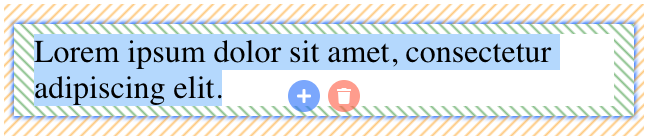
\includegraphics[width=3in]{../editframe.png}
  \caption{The edit frame shown in the WYSIWYG editor, highlighting the selected element. Margins (outside of the element) are highlighted in yellow and padding (inside of the element) are highlighted in green.}
  \label{fig:editframe}
\end{figure}

\subsection{Properties Editor}
The Properties Editor shows information about the currently selected definition / data, and allows the user to modify properties about these objects such as HTML attributes and styles.

The properties editor is organized into various tabs where the user can modify different aspects of the selected content. There are 4 potential tabs that may be shown depending on the current selection:
\begin{itemize}
  \item \textbf{Element:} When an HTML element is selected, this tab displays properties about that element such as the tag name and attributes. The user can modify all of these (with the exception of the tags on \texttt{head} and \texttt{body} elements, which cannot be changed, though attributes on these elements are still modifiable).
  \item \textbf{Component:} When a component definition is selected (in the first step of the Navigator), this tab gives the user a way to rename the component. When a component reference (inside of a page or component definition) is selected, this tab allows the user to choose another component to reference instead.
  \item \textbf{Text:} When a piece of text is selected, this tab gives the user another way of editing the text content.
  \item \textbf{Style:} This tab is always shown, but shows slightly different things depending on the selection. For example, if an element is selected, only the style rules that apply to that element will be shown. If a page is selected, but no data within that page is selected, all style rules will be shown. Text selections will show the style rules for their parent element, and component selections will show the style rules for their root element.
\end{itemize}

The properties editor makes use of various user-friendly inputs in order to assist novice users. For example, the editor makes heavy use of a 'combo-box' style input. This allows the user to both type text freely, or to select from a pre-defined list of curated values. This provides power to more technical users, such as developers, who may wish to enter a value other than those which have been pre-defined, while providing an easy-access option to novice users who may not otherwise know what values can be used.

\section{Implementation}
Loom is implemented using TypeScript\cite{TypeScript} and the Electron\cite{Electron} framework. Implementing Loom using web technologies enables a high level of code reuse, and means that Loom can take advantage of Web APIs in order to implement some features, simplifying the codebase. The Electron framework enables web applications to act as native applications by making native APIs available to scripts running in a pre-packaged web browser. Electron has built-in cross-platform support, meaning that Loom works across Mac, Windows, and Linux.

The implementation of Loom is divided into two primary packages: the UI, and the "Core".

\subsection{Core}
The Core portion of Loom contains the underlying data structures used to implement Loom's features. These are conceptually divided into two halves: definitions, or source data, which is the data the user directly modifies with Loom, and "built" data, which corresponds directly with web technologies such as HTML and CSS. The separation of the two halves enables abstractions. For example, components only exist within definitions, and get replaced with their corresponding elements (thereby duplicating the elements) within built objects.

The build process to transform Definitions into Built Objects is "reactive". That is, a set of Built Objects (collectively called Results) automatically updates along with the corresponding Definitions (collectively called Sources), so that if any value within the Sources change, the Results will update appropriately as well. To enable this reactive connection, Loom makes heavy use of event-driven programming, including a collection of event-driven data structures specifically created for use within Loom, creatively titled "Loom Data".

\begin{figure}[!t]
  \centering
  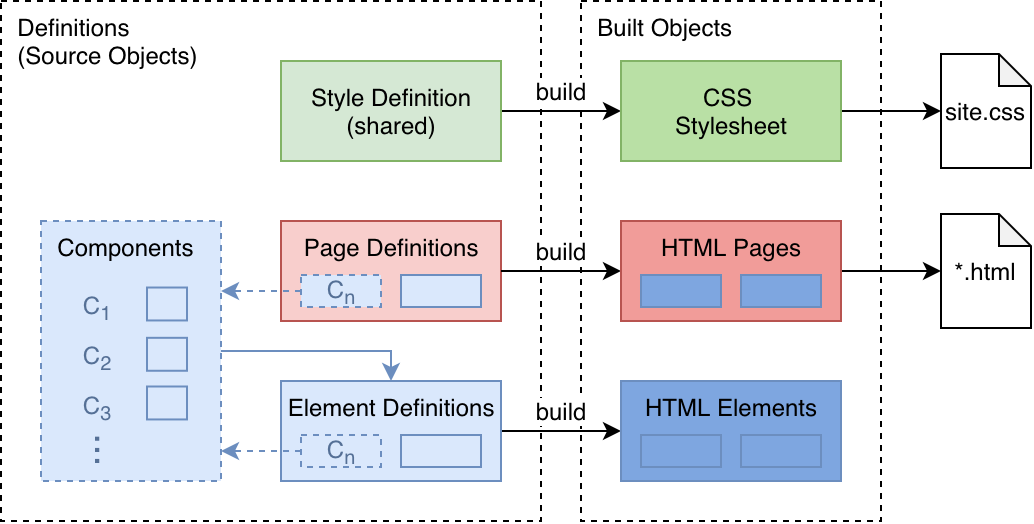
\includegraphics[width=3in]{../core.png}
  \caption{Connections between Definitions, Built Objects, and outputs of Loom}
  \label{fig:core}
\end{figure}

Figure \ref{fig:core} shows the relationship between each basic type of Definition and its corresponding Built Object. Page and Element Definitions can both make use of Component references, but their corresponding Built Objects cannot -- the references must be replaced with concrete Elements.

\subsection{UI}
The UI implements all GUI aspects of Loom using the Electron framework. The primary function of the UI is to display the data from Built Objects and allow the user to modify the corresponding data within Definitions. The resulting data flow is similar to that of an MVC architecture (where Built Objects are the model and Definitions take the place of a Controller) and helps maintain a logical separation between the UI and Core. Figure \ref{fig:dataflow} visualizes this data flow.

Due to the heavy use of event-driven programming and custom data structures within Loom Core, the UI portion of loom does not use any UI frameworks such as React\cite{React} -- instead using a custom solution that is designed to work well with the event-driven behavior and data structures present in Loom Core.

Every component within the UI inherits from a base class that enables components to emit events, manage their child components, and define lifecycle behaviors for creation and destruction. This allows components to easily watch for events from a data source, update their contents when events happen, and remove any event listeners when they get destroyed (a very common pattern).

The root component of the UI also stores global states such as the loaded project and selected data. Many components within the UI read and modify this data in order to implement their behavior -- for example, the Navigator reads and modifies the selected data, and the Properties editor reads the selected data to determine what to display. Events are emitted whenever these values change, so that components can update themselves accordingly.

\begin{figure}[!t]
  \centering
  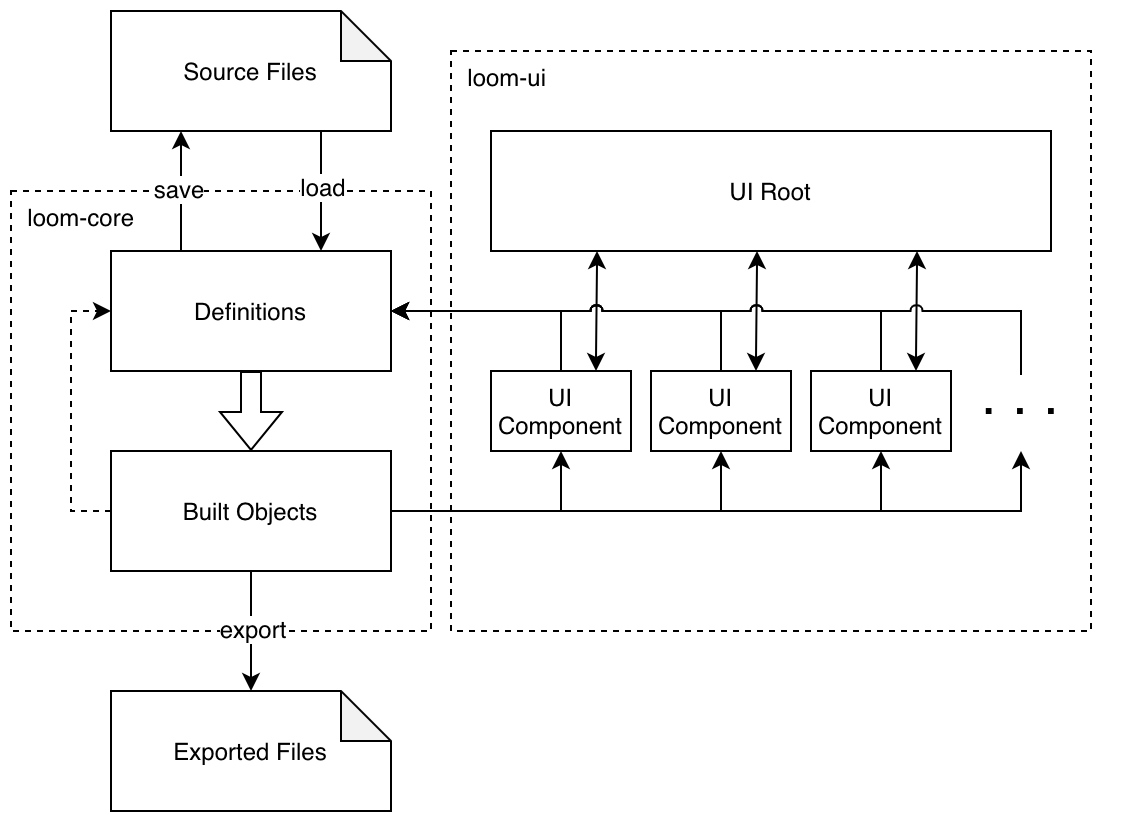
\includegraphics[width=3in]{../dataflow.png}
  \caption{Flow of data / events within Loom Core and UI.}
  \label{fig:dataflow}
\end{figure}

\subsection{Serialization / Deserialization}
Loom allows the user to save \& load projects, and export projects to web-ready files. File formats and structures are specified for both of these functions.

A saved project is a directory consisting of:
\begin{itemize}
  \item A "pages" or "src" directory, containing all of the pages in the project. These are XHTML format, except for component references, which use the XML namespace '\texttt{loom:}' to differentiate themselves from HTML elements.
  \item A "components" directory, containing all of the components in the project. The name of each html file in this directory determines the name of the component, with the root element in each file being the root element for that component.
  \item A "loom.json" file, containing metadata about the project. At present this may specify custom paths for the pages and components directories.
\end{itemize}

When a project is exported, its contents are built and the built objects are serialized into output files. All pages, as well as the global stylesheet, are output into a shared root directory. Pages are in standard HTML format and the stylesheet is in standard CSS format.

\section{Evaluation}
To evaluate how well Loom achieves its goals, we evaluate the ability to perform various target tasks from the point of view of each category of user, including novice users, developers, and designers.

\begin{table*}[!t]
\renewcommand{\arraystretch}{1.3}
\caption{Evaluated Goals for Novice Users}
\label{table:novice_goals}
\centering
\begin{tabular}{|r|c|p{8cm}|}
\hline
Goal & Evaluation & Comments \\
\hline \hline
Create and Delete Pages & \textbf{\color{ForestGreen}good} & "Add Page" button is shown when choosing a page. Deletion controls are available in right-click menu and Properties editor when a page is selected \\
\hline
Create and Delete Elements & \textbf{\color{ForestGreen}good} & Controls for creation are shown in the navigator and WYSIWYG editor. Controls for deletion are shown in all three parts of the interface \\
\hline
Bold / Italic / Underline Text & \textbf{\color{Dandelion}fair} & Keyboard shortcuts are supported, but no interface controls that novice users would be familiar with \\
\hline
Create Images / Links & \textbf{\color{Red}poor} & Images are currently unsupported. Links are not very user-friendly \\
\hline
Set Basic Styles & \textbf{\color{Dandelion}fair} & Search functionality and friendly style choosers for some styles, but not all -- and CSS style names may not be obvious to novice users \\
\hline
Save Project as Static Pages & \textbf{\color{ForestGreen}good} & Export option within "File" menu allows exporting sites in a few clicks \\
\hline
Associate Visual Content with HTML & \textbf{\color{ForestGreen}good} & Selected text / Elements are highlighted in the WYSIWYG editor and update immediately when modified \\
\hline
Associate Visual Content with CSS & \textbf{\color{Dandelion}fair} & Changes made to styles can be seen immediately within the WYSIWYG editor, but this is currently the only way to associate styles on the page with the CSS rules applying them  \\
\hline
Get Help with HTML & \textbf{\color{Red}poor} & There is currently no help text for HTML elements, attributes, etc. \\
\hline
Get Help with CSS & \textbf{\color{Dandelion}fair} & CSS properties have a "help text" icon that shows information about the property when clicked. However, this help is technical and may not be entirely useful for novice users \\
\hline
\end{tabular}
\end{table*}

\begin{table*}[!t]
  \renewcommand{\arraystretch}{1.3}
  \caption{Evaluated Goals for Developers}
  \label{table:developer_goals}
  \centering
  \begin{tabular}{|r|c|p{8cm}|}
    \hline
    Goal & Evaluation & Comments \\
    \hline \hline
    Set Custom HTML Attributes & \textbf{\color{ForestGreen}good} & A key-value entry interface within the Properties editor allows users to edit arbitrary HTML attributes \\
    \hline
    Set Custom CSS Property values & \textbf{\color{Dandelion}fair} & Arbitrary CSS properties can be set within the Style tab of the Properties editor. However, some aspects of CSS such as media queries are currently unsupported \\
    \hline
    View Properties of an Element & \textbf{\color{ForestGreen}good} & A key-value interface within the Properties editor displays all set properties of the selected element \\
    \hline
    View Styles for an Element & \textbf{\color{ForestGreen}good} & All CSS styles can be viewed within the Propertied editor. In addition, when an emelemt is selected, only style rules which apply to that element are shown \\
    \hline
    Create Custom CSS Rules & \textbf{\color{Dandelion}fair} & Creation of CSS rules with arbitrary selectors is supported. However, some aspects of CSS such as media queries are currently unsupported \\
    \hline
    Create and Edit Scripts & \textbf{\color{Red}poor} & Currently unsupported \\
    \hline
  \end{tabular}
\end{table*}

\begin{table*}[!t]
  \renewcommand{\arraystretch}{1.3}
  \caption{Evaluated Goals for Designers}
  \label{table:designer_goals}
  \centering
  \begin{tabular}{|r|c|p{8cm}|}
    \hline
    Goal & Evaluation & Comments \\
    \hline \hline
    Create Elements Quickly & \textbf{\color{ForestGreen}good} & There are several ways to create new elements \\
    \hline
    See Immediate Output & \textbf{\color{ForestGreen}good} & Any time the content or style of any element is changed, the WYSIWYG editor immediately updates to display the change \\
    \hline
    Layout Content Quickly & \textbf{\color{Red}poor} & Organizing content on the page is currently a very "manual" process -- involving creating elements and tweaking their CSS layout properties. Elements also cannot be moved from within the WYSIWYG editor \\
    \hline
    Create Flows Across Pages & \textbf{\color{Red}poor} & Currently unsupported \\
    \hline
    Modify Font Styles & \textbf{\color{Dandelion}fair} & CSS properties allow modification of font styles, however finding the correct properties to apply may be a frustrating process for designers \\
    \hline
    Set Padding and Margins & \textbf{\color{Dandelion}fair} & CSS properties allow modification of padding and margins, however there is currently no "friendly" interface for this and so this may be frustrating to designers \\
    \hline
    Copy and Tweak Existing Pages & \textbf{\color{Red}poor} & Currently unsupported \\
    \hline
    Palette of Standard Colors & \textbf{\color{Red}poor} & Currently unsupported \\
    \hline
  \end{tabular}
\end{table*}

\subsection{Novice Users}
Novice users include those who have little knowledge about web technologies, and potentially minimal experience with other web design tools. We do however assume that they are experienced web users in general. Loom aims to give these users the ability to accomplish simple tasks with little or no frustration. The evaluated goals for novice users are shown in Table \ref{table:novice_goals}.


\subsection{Developers}
Developers may already be familiar with web technologies, or may just be learning them. In either case, Loom aims to give power to these users and enable rapid prototyping. The evaluated goals for developers are shown in Table \ref{table:developer_goals}.

\subsection{Designers}
Designers are less interested in the underlying workings of a layout, and are instead looking for a way to rapidly create layouts and style components before they hand it off to a developer. The evaluated goals for designers are shown in Table \ref{table:designer_goals}.


\section{Conclusion}
Loom aims to fill a void in current web development applications by allowing users of various backgrounds to develop web sites using one unified tool. This would improve collaboration among users of different backgrounds, such as novices, developers, and designers, as well as acting as a learning tool for those who are unfamiliar with web technologies -- teaching common concepts about web technologies that users can apply to other tools or even to understanding / writing web code.

Loom does not currently achieve all of its goals, even among those that have been evaluated, showing that there is room for improvement. Nonetheless, we have demonstrated the potential for Loom to be a useful tool for a wide variety of users with differing backgrounds and needs. The foundation of Loom is flexible enough to support additional features to further achieve these goals.


\section{Future Work}
There is much future work to be done on Loom. At present, the user interface is not as user-friendly as it could be. Several features could improve the experience for beginner users:
\begin{itemize}
  \item Additional drag-and-drop features, such as the ability to create new elements by dragging from a list of pre-made elements
  \item Additional controls within the WYSIWYG editor, such as the ability to modify styles of a selected element or text
  \item Additional help text, such as to explain available HTML attributes, CSS selectors, and CSS properties
  \item Improved interface for creating and editing CSS selectors and rules in general
  \item Better UI for renaming pages and organizing site structure
  \item Other general bugfixes and UX improvements
\end{itemize}

Further evaluation of Loom such as user trials could also help identify additional areas for improvement.

\medskip

In addition to usability improvements, there are several additional features the author has considered, but deferred for this initial prototype of Loom:
\begin{itemize}
  \item Parameterized components, where uses of a component can pass "variables" such as text or child components for use within the component definition
  \item Support for media files, such as images or custom fonts
  \item Support for scripts and script editing within Loom
  \item Support for multiple stylesheets, and editing of inline / external stylesheets
  \item Automatic linking between pages -- for example, if the location of a page is modified, other pages which link to that page will automatically have their references updated
  \item The ability to import an existing website into Loom
  \item Custom attributes, such as animations, which would have complex compilation rules to determine how the value of the attribute affects other values such as HTML attributes and styles.
  \item Post-processing of output content, such as automatically shortening class names, polyfilling CSS code for cross-browser support, or minifying / inlining CSS and scripts.
  \item Creation of a CLI tool to allow Loom projects to be built without the use of the UI.
  \item Integration of version control tools, enabling Loom to be used by many users collaborating together on one project.
  \item Integration of deployment services such as Netlify\cite{Netlify}, enabling Loom to be used like a Content Management System.
\end{itemize}

\pagebreak

% conference papers do not normally have an appendix


% use section* for acknowledgement
% \section*{Acknowledgment}
% The authors would like to thank...





% trigger a \newpage just before the given reference
% number - used to balance the columns on the last page
% adjust value as needed - may need to be readjusted if
% the document is modified later
%\IEEEtriggeratref{8}
% The "triggered" command can be changed if desired:
%\IEEEtriggercmd{\enlargethispage{-5in}}

% references section

% can use a bibliography generated by BibTeX as a .bbl file
% BibTeX documentation can be easily obtained at:
% http://www.ctan.org/tex-archive/biblio/bibtex/contrib/doc/
% The IEEEtran BibTeX style support page is at:
% http://www.michaelshell.org/tex/ieeetran/bibtex/


\bibliographystyle{IEEEtran}
\bibliography{IEEEabrv,report}


% argument is your BibTeX string definitions and bibliography database(s)
%\bibliography{IEEEabrv,../bib/paper}
%
% <OR> manually copy in the resultant .bbl file
% set second argument of \begin to the number of references
% (used to reserve space for the reference number labels box)
% \begin{thebibliography}{1}
%
% \bibitem{IEEEhowto:kopka}
% H.~Kopka and P.~W. Daly, \emph{A Guide to \LaTeX}, 3rd~ed.\hskip 1em plus
%   0.5em minus 0.4em\relax Harlow, England: Addison-Wesley, 1999.
%
% \end{thebibliography}




% that's all folks
\end{document}


